\documentclass{beamer}
\usepackage{color}
\usepackage{subfig}
\usepackage{graphicx}
\usepackage{float}
\usepackage{cite}
\usepackage{bbm}
\usepackage{comment}
%\usepackage[UTF8]{ctex}
\usepackage{tikz}
\usepackage{scalefnt, xr}
\usetikzlibrary{arrows}
\usetikzlibrary{plotmarks}
\usetikzlibrary{overlay-beamer-styles}
\usetikzlibrary{calc}
\usetikzlibrary{scopes}
\usetheme{Madrid}
\usepackage{tikz}
\usetikzlibrary{arrows.meta,decorations.pathmorphing}

\theoremstyle{plain}
\newtheorem{thm}{Theorem}
\newtheorem{cor}[thm]{Corollary}
\newtheorem{lem}[thm]{Lemma}
\newtheorem{prop}[thm]{Proposition}
\newtheorem{remark}[thm]{Remark}
%
\theoremstyle{definition}
\newtheorem{defn}[thm]{Definition}


\colorlet{prp}{red!50!blue!80!white}
\colorlet{Tcol}{blue}
\colorlet{Fcol}{orange!85!red!90!black}
\colorlet{rgr}{red!70!gray}
\colorlet{bgr}{blue!60!gray}
\colorlet{gray}{black!50!white}
\colorlet{lgray}{gray!50!white}
\colorlet{dfc}{green!35!blue!80!gray!90!black}
\colorlet{rfc}{black!45!gray!80!blue!80!white}
\colorlet{rkc}{lightgray}
\colorlet{rsbcol}{green!80!blue!70!gray!70!black}
\colorlet{nbdcol}{red!60!blue!90!gray!90!black}
\newcommand{\BB}{\mathbbm}
\newcommand{\ol}{\overline}
\newcommand{\ul}{\underline}
\newcommand{\op}{\operatorname}
\newcommand{\la}{\langle}
\newcommand{\ra}{\rangle}
\newcommand{\bd}{\mathbf}
\newcommand{\im}{\operatorname{Im}}
\newcommand{\re}{\operatorname{Re}}
\newcommand{\frk}{\mathfrak}
\newcommand{\eqD}{\overset{d}{=}}
\newcommand{\ep}{\varepsilon}
\newcommand{\rta}{\rightarrow}
\newcommand{\xrta}{\xrightarrow}
\newcommand{\Rta}{\Rightarrow}
\newcommand{\hookrta}{\hookrightarrow}
\newcommand{\wt}{\widetilde}
\newcommand{\wh}{\widehat} 
\newcommand{\mcl}{\mathcal}
\newcommand{\pre}{{\operatorname{pre}}}
\newcommand{\lrta}{\leftrightarrow}
\newcommand{\bdy}{\partial} 
\newcommand{\rng}{\mathring}
\newcommand{\srta}{\shortrightarrow}
\newcommand{\el}{l}
\newcommand{\ER}{Erd\H{o}s-R\'{e}nyi\ }
\newcommand{\tr}{{\mathrm{tr}}}
\newcommand{\LFPP}{{\textnormal{\tiny{\textsc{LFPP}}}}}
\newcommand{\ccM}{{\mathbf{c}_{\mathrm M}}}
\newcommand{\Pb}{\mathbb P}
\newcommand{\Qb}{\mathbb Q}

\newcommand{\red}{\textcolor{red}}
\newcommand{\blue}{\textcolor{blue}}
\newcommand{\cyan}{\textcolor{cyan}}

\newcommand*\tc[1]{\tikz[baseline=(char.base)]{\node[shape=circle,draw,inner sep=1pt] (char) {#1};}}
\newcommand*\tb[1]{\tikz[baseline=(char.base)]{\node[shape=rectangle,draw,inner sep=2.5pt] (char) {#1};}}

%Remove spacing before \left and \right
\let\originalleft\left
\let\originalright\right
\renewcommand{\left}{\mathopen{}\mathclose\bgroup\originalleft}
\renewcommand{\right}{\aftergroup\egroup\originalright}



\newcommand{\post}[2]{\begin{center} \includegraphics[width=#2]{#1} \end{center} }
\newcommand{\scite}[1]{\textcolor{blue}{\scriptsize [#1]}}

%Information to be included in the title page:
\title[Algorithmic Contiguity]{Algorithmic Contiguity from Low-degree Conjecture and Applications in Correlated Random Graphs}
\author[Zhangsong Li]{Zhangsong Li}
\institute[]{School of Mathematical Sciences, Peking University}
\date[August 2025]{August 12, 2025 \\ \medskip\bigskip\bigskip
International Conference on Randomization and Computation }


\begin{document}

\frame{\titlepage}





\begin{frame}
\frametitle{Graph matching (graph alignment)}

\begin{center}
\begin{tikzpicture}
[baseline=1em,scale = 1,
main node/.style={circle,draw,minimum size=18pt,inner sep=1pt,font=\sffamily\Large\bfseries}]
\pgfmathsetseed{30}

\def\r{1.5}
\def\n{10}
\def\x{6}

\foreach \i in {1,...,\n}{
%\pgfmathsetmacro\r{0.2+rnd*0.8}
% \pgfmathsetmacro\a{rnd*360}
\only<1>
 {\node[main node, fill=blue!60]  (a\i) at ( {\r*cos(360*\i/\n)} ,  { \r*sin(360*\i/\n) } ){};
 \node[main node, fill=blue!60]  (b\i) at ( {\x+\r*cos(360*\i/\n)} ,  {\r*sin(360*\i/\n) } ){};
 }
 \only<2->
 {\node[main node, fill=blue!60]  (a\i) at ( {\r*cos(360*\i/\n)} ,  { \r*sin(360*\i/\n) } ){$\pgfmathprint{int(\i-1)}$};
 \node[main node, fill=blue!60]  (b\i) at ( {\x+\r*cos(360*\i/\n)} ,  {\r*sin(360*\i/\n) } ){$\pgfmathprint{int(\i-1)}$};
 }
 %{$\i$};

 }

 \foreach \i in{1,..., \n}
 {
  \foreach \j in{ \i,..., \n}
  {
      \pgfmathparse{rnd>0.2}
           \ifnumcomp{\pgfmathresult}{=}{1}
           {

            \pgfmathparse{rnd>0.4}
            \ifnumcomp{\pgfmathresult}{=}{1}{
    \draw [black] (a\i) -- (a\j);}

            \pgfmathparse{rnd>0.4}
            \ifnumcomp{\pgfmathresult}{=}{1}{
    \draw [black] (b\i) -- (b\j);}

  }

   }
   }
\end{tikzpicture}
\end{center}
\vspace{1\baselineskip}
\pause $\bullet$ Goal: find a \blue{bijection} between two vertex sets that maximally align the edges (i.e.~minimizes $\#$ of adjacency disagreements).

\medskip

\pause $\bullet$ Since graph alignment is \blue{NP-hard} to solve/approximate in worst case, we instead consider some \blue{average-case models}.



\end{frame}










\begin{frame}
\frametitle{An idealized model: correlated \ER graphs model}

\begin{center}
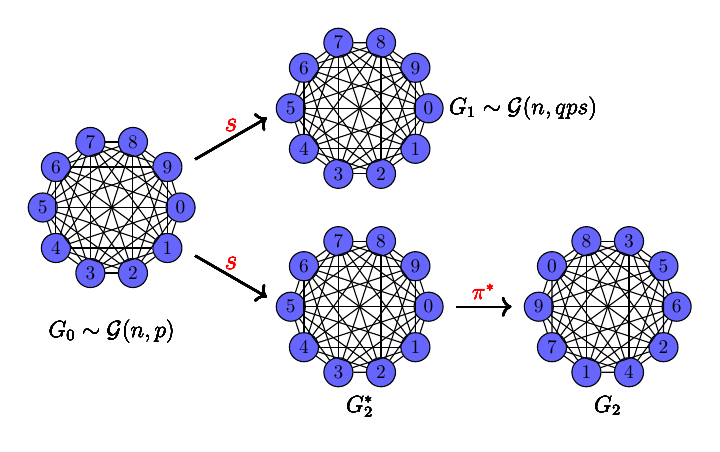
\begin{tikzpicture}
[baseline=1em,scale = 0.7,transform shape,
main node/.style={circle,draw,minimum size=15pt,inner sep=1pt
%font=\sffamily\Large\bfseries
}]
\pgfmathsetseed{30}

\def\r{1.25}
\def\n{10}
\def\x{4.5}
\def \y{1.8}
\def \z{{6,2,4,1,7,9,0,8,3,5}}
\def \w{{7,4,2,9,3,10,1,5,8,6}}

\foreach \i in {1,...,\n}{
%\pgfmathsetmacro\r{0.2+rnd*0.8}
% \pgfmathsetmacro\a{rnd*360}
\node[main node, fill=blue!60]  (a\i) at ( {\r*cos(360-360*(\i-1)/\n)} ,  { \r*sin(360-360*(\i-1)/\n) } ){$\pgfmathprint{int(\i-1)}$};
\node at (0, {-1-\r}){\large $G_0 \sim \mathcal G(n,p)$};
\uncover<2->
{
\draw[->,thick,black] ({(\r+0.5)*cos(30)  }, {(\r+0.5)*sin(30)}) -- ({(\r+2)*cos(30)  }, {(\r+2)*sin(30)});
\node[red,above]  at ({(\r+1.25)*cos(30)  }, {(\r+1.25)*sin(30)}){\Large $s$};

\node[right]  at ({\x+\r+0.25}, \y){\large $G_1\sim \mathcal G(n,q\triangleq ps)$};

\node[main node, fill=blue!60]  (b\i) at ( {\x+ \r*cos(360-360*(\i-1)/\n)} ,  { \y+\r*sin(360-360*(\i-1)/\n) } ){$\pgfmathprint{int(\i-1)}$};
}
\uncover<3->
{

\draw[->,thick,black] ({(\r+0.5)*cos(-30)  }, {(\r+0.5)*sin(-30)}) -- ({(\r+2)*cos(-30)  }, {(\r+2)*sin(-30)});
\node[red,above]  at ({(\r+1.25)*cos(-30)  }, {(\r+1.25)*sin(-30)}){\Large $s$};

\node[below]  at ({\x}, {-\y-\r-0.25} ){\large $G_2^*$};

\node[main node, fill=blue!60]  (c\i) at ( {\x+\r*cos(360-360*(\i-1)/\n)} ,  {\r*sin(360-360*(\i-1)/\n) - \y } ){$\pgfmathprint{int(\i-1)}$};
}
\uncover<4->
{
  \draw[->,thick,black] ( {\x+\r+0.5 } , {-\y} ) -- ({\r+1.5+\x   }, {-\y});
  \node[above,red] at ( {\x+\r +1.0}, {-\y}) {\large $\pi^*$};
  \node[below]  at ({2*\x}, {-\y-\r-0.25} ){\large $G_2$};
  \pgfmathsetmacro\l{\z[\i-1]};
 %\node[main node, fill=blue!60]  (d\i) at ( {2*\x+\r*cos(360-360*(\z[\i-1]-1)/\n)} ,  {\r*sin(360-360*(\z[\i-1]-1)/\n) - \y } ){$\l$};
  \node[main node, fill=blue!60]  (d\i) at ( {2*\x+\r*cos(360-360*(\i-1)/\n)} ,  {\r*sin(360-360*(\i-1)/\n) - \y } )
  {$\l$};
}



 }

 \foreach \i in{1,..., \n}
 {
  \foreach \j in{ \i,..., \n}
  {
      \pgfmathparse{rnd>0.2}
           \ifnumcomp{\pgfmathresult}{=}{1}
           {
            \draw [black] (a\i) -- (a\j);

            \pgfmathparse{rnd>0.4}
            \ifnumcomp{\pgfmathresult}{=}{1}{
    \uncover<2->{\draw [black] (b\i) -- (b\j);}
    }

            \pgfmathparse{rnd>0.4}
            \ifnumcomp{\pgfmathresult}{=}{1}{
    \uncover<3->{\draw [black] (c\i) -- (c\j);}
    
    \uncover<4->{
    \pgfmathparse{\w[\i-1]}\let\firstnode\pgfmathresult
    \pgfmathparse{\w[\j-1]}\let\secondnode\pgfmathresult
    \draw [black] (d\firstnode) -- (d\secondnode);
     }

  }

   }
   }
   }
\end{tikzpicture}
\end{center}

\pause \pause \pause

\pause Marginal edge density: $q=ps$; edge correlation: $\rho=\tfrac{s(1-p)}{1-ps}$.

\end{frame}






\begin{frame}
\frametitle{Information thresholds and efficient algorithms}

{\bf Three} inference tasks: \blue{detection}, \blue{exact recovery}, \blue{partial recovery}.

$\bullet$ \blue{Detection}: test correlation against independence.

$\bullet$ \blue{Exact recovery}: correctly match all vertices.

$\bullet$ \blue{Partial recovery}: correctly match a positive fraction of vertices.

\medskip

\pause We will focus on the \blue{sparse} regime where $q=n^{-1+o(1)}$.

\medskip

\pause \red{[Wu-Xu-Yu'23][Ding-Du'22,23][Feng'25]}: Detection/partial recovery (respectively, exact recovery) is information-theoretically possible if and only if $\rho>\tfrac{1}{nq}\wedge\sqrt{\alpha}$ (respectively, $\rho>\tfrac{\log n}{nq}$), where $\alpha\approx 0.338$ is the Otter's constant.

\medskip

\pause \red{[Mao-Wu-Xu-Yu'21,23][Ganassali-Massouli\'e-Lelarge'23,24]}: Detection/partial recovery is possible by efficient algorithms if $\rho>\sqrt{\alpha}$; exact recovery is possible if $\rho>\sqrt{\alpha}$ and $nq>\log n$.



\end{frame}







\begin{frame}
\frametitle{The low-degree polynomial framework}

\small

\pause $\bullet$ {\bf Degree-$D$ test}: multivariate polynomials $f: \{ 0,1 \}^{2\times \binom{n}{2}} \longrightarrow \mathbb R$ of degree $D=D_n$

\medskip

\pause $\bullet$ ``Success'': $f=f_n$ \blue{strongly/weakly separates} $\Pb$ and $\Qb$ if
\begin{equation*}
    \sqrt{ \max\{ \operatorname{Var}_{\Pb}(f), \operatorname{Var}_{\Qb}(f) \} } = \blue{o(1)/O(1)} \cdot \big| \mathbb E_{\Pb}[f] - \mathbb E_{\Qb}[f] \big| \,. 
\end{equation*}

\pause $\bullet$ Heuristics: failure of degree-$D$ polynomials $\Longrightarrow$ failure of algorithms with running time $n^{D/\operatorname{polylog}(n)}$.

\medskip

\pause $\bullet$ Usually prove the ``failure'' of degree-$D$ polynomials by showing the following bound on the low-degree advantage for some $\operatorname{TV}(\Pb,\Pb'),\operatorname{TV}(\Qb,\Qb')=o(1)$:
\begin{align*}
    \mathsf{Adv}_{\leq D}(\Pb',\Qb'):= \max_{ \operatorname{deg}(f) \leq D } \frac{ \mathbb E_{\Pb'}[f] }{ \sqrt{\mathbb E_{\Qb'}[f^2]} } = \blue{O(1)/1+o(1)}
\end{align*}

\pause \red{[Ding-Du-L.'23]}: $\mathsf{Adv}_{\leq D}(\Pb',\Qb')=O(1)$ when $\rho<\sqrt{\alpha}$ and $D=\exp\big( o(\tfrac{\log n}{\log nq}) \big)$.

\medskip

\pause $\bullet$ This suggests that detection is ``hard''. What about \blue{partial recovery}?

\end{frame}







\begin{frame}{Our results}

We say a family of estimators $\{ h_{i,j}: 1 \leq i,j \leq n \}$ ($h_{i,j}$ estimates $\mathbf 1_{\pi_*(i)=j}$) achieves partial recovery if
\begin{itemize}
    \item $h_{i,j} \in \{ 0,1 \}$ for all $i,j$ w.h.p. under $\Pb$.
    \item $h_{i,1}+\ldots +h_{i,n}=1$ for all $i$ w.h.p. under $\Pb$.
    \item $\Pb( \sum_{1 \leq i \leq n} h_{i,\pi_*(i)} \geq \Omega(n) ) \geq \Omega(1)$.
\end{itemize}

\pause
\begin{theorem}[L.'2025+, informal]
    Assuming low-degree conjecture, for the correlated \ER model $\mathcal G(n,q,\rho)$, when $q=n^{-1+o(1)}$ and $\rho<\sqrt{\alpha}$ all estimators $\{ h_{i,j} \}$ that achieves partial recovery requires running time $n^{D/\operatorname{polylog}(n)}$, where $D=\exp\big( o(\tfrac{\log n}{\log nq}) \big)$. 
\end{theorem}

\end{frame}






\begin{frame}
\frametitle{Ingredient: algorithmic contiguity}

\pause \red{[Ding-Du-L.'23]}: for any $\rho<\sqrt{\alpha}$ and any $D=D_n=\exp\Big( o\big( \tfrac{\log n}{\log nq} \big) \Big)$, 
\begin{equation*}
    \mathsf{Adv}_{\leq D}(\Pb',\Qb')=O(1) \mbox{ for some } \operatorname{TV}(\Pb,\Pb'), \operatorname{TV}(\Qb,\Qb')=o(1) \,.
\end{equation*}

\pause $\bullet$ ``Standard'' low-degree conjecture: \blue{strong detection} requires time $\exp(D/\operatorname{polylog}(n))$.

\medskip

\pause $\bullet$ {\bf Improvement} (algorithmic contiguity): any \blue{one-sided detection} algorithm $\mathcal A=\mathcal A_n$ such that 
\begin{equation*}
    \Pb(\mathcal A=1)=\Omega(1) \,, \quad \Qb(\mathcal A=0)=1-o(1)
\end{equation*}
requires running time $\exp(D/\operatorname{polylog}(n))$.

\end{frame}






\begin{frame}{Proof of algorithmic contiguity}

\begin{itemize}
    \item<1-> Assume on the contrary that an algorithm $\mathcal A$ such that $\Pb(\mathcal A=1)=\Omega(1)$ and $\Qb(\mathcal A=0)=1-\epsilon$ where $\epsilon=\epsilon_n\to 0$. WLOG $\epsilon_n \geq 1/\operatorname{poly}(n)$. 
    \item<2-> Let $M=M_n=\epsilon_n^{-1/2}$ and consider the following detection problem: 
    \begin{itemize}
        \item $\widehat{\Qb}=\Qb^{ \otimes M }$; 
        \item $\widehat{\Pb}=$ law of $(Y_1,\ldots,Y_M)$ s.t. $Y_{\kappa} \sim \Pb$ and $Y_j \sim \Qb: j \neq \kappa$ for some $\kappa \in \operatorname{unif}([M])$;
    \end{itemize}
    Then $\widehat{\Qb}( (\mathcal A(Y_1), \ldots \mathcal A(Y_M))=(0,\ldots,0) )=1-o(1)$ and $\widehat{\Pb}( (\mathcal A(Y_1), \ldots \mathcal A(Y_M)) \neq (0,\ldots,0) )=\Omega(1)$.
    \item<3-> However, $\mathsf{Adv}_{\leq D}(\Pb,\Qb)=O(1) \Longrightarrow$ $\mathsf{Adv}_{\leq D}(\widehat\Pb,\widehat\Qb)=1+o(1)$, which leads to contradiction.
\end{itemize}

\end{frame}







\begin{frame}{Hardness of partial recovery: proof idea}

\begin{itemize}
    \item<1-> Assume on the contrary that $\{ h_{i,j} \}$ achieves partial recovery. WLOG $h_{i,j} \in \{ 0,1 \}$ and $\cyan{\sum_{1 \leq j \leq n} h_{i,j} \in \{ 0,1 \}}$ hold for all realizations.
    \item<2-> We expect that
    \begin{align*}
        & \{ h_{i,j} \} \mbox{ achieves partial recovery } \\
        \Longrightarrow\ & \Pb( h_{i,\pi_*(i)}=1 )=\Omega(1) \mbox{ for some } i \\
        \Longrightarrow\ & \Pb(h_{i,j}=1 \mid \pi_*(i)=j)=\Omega(1) \mbox{ for } \Omega(n) \mbox{ number of } j \,.
    \end{align*}
    \item<3-> We can show that $\mathsf{Adv}_{\leq D}( \Pb(\cdot\mid \pi_*(i)=j), \Qb )=O(1)$ (similar to the detection lower bound). Thus \blue{algorithmic contiguity} implies that $\Qb( h_{i,j}=1 ) \geq \Omega(1)$. 
    \item<4-> Yields $\mathbb E_{\Qb}[ \sum_{1 \leq j \leq n} h_{i,j} ]=\Omega(n)$, contradiction to \cyan{$(*)$}!
\end{itemize}

\end{frame}







\begin{frame}{Summary and future perspectives}

\begin{itemize}
    \item We know that in sparse correlated \ER graphs, detection is easy when the correlation $\rho>\sqrt{\alpha}$ and hard when $\rho<\sqrt{\alpha}$. But what about partial recovery?
    \item Assuming low-degree conjecture, we found a reduction from partial recovery to detection. Thus partial recovery is also hard when $\rho<\sqrt{\alpha}$.
    \item Key ingredient: developing ``algorithmic contiguity'' between two probability measures from bounded low-degree advantage.
    \item Open: more ``direct'' analysis for low-degree hardness for partial recovery?
\end{itemize}

\underline{Reference}: 

Zhangsong Li. Algorithmic Contiguity and Applications in Correlated Random Graphs. arXiv:2502.09832v3.



\end{frame}












%\begin{frame}
%\frametitle{A more realistic variant: stochastic block model}

%\begin{center}
%\begin{tikzpicture}
%[baseline=1em,scale = 0.7,transform shape,
%main node/.style={circle,draw,minimum size=15pt,inner sep=1pt
%font=\sffamily\Large\bfseries
%}]
%\pgfmathsetseed{30}

%\def\r{1.25}
%\def\n{10}
%\def\x{4.5}
%\def \y{0}
%\def \z{{-1,-1,1,1,-1,1,1,-1,-1,1}}
%\edef\setA{{1,5,3,0,8}}
%\edef\setB{{2,4,6,7,9}}

%\foreach \i in {1,...,\n}{
%\pgfmathsetmacro\r{0.2+rnd*0.8}
% \pgfmathsetmacro\a{rnd*360}
%\node[main node, fill=blue!60]  (a\i) at ( {-0.5+\r*cos(360-360*(\i-1)/\n)} ,  { \r*sin(360-360*(\i-1)/\n) } ){$\pgfmathprint{int(\i-1)}$};
%\node at (-0.5, {-0.5-\r}){\large $V$};
%\uncover<2->
%{

%\draw[->,thick,black] ( {\x-3.25} , {-\y} ) -- ({\x+0.25   }, {-\y});
%  \node[above,red] at ( {\x-1.5}, {-\y}) {\large $\text{uniform labeling}$};
%  \node[below,red] at ( {\x-1.5}, {-\y}) {\large $\sigma_i \sim \mathsf{Unif}(\{-1, 1\})$};

%\node[below]  at ({2+\x}, {-\y-\r-0.25} ){\large $V_{\text{labeled}}$};
%\pgfmathparse{int(\z[\i-1])}
%\ifnum\pgfmathresult=1
%    \node[main node, fill=blue!60]  (c\i) at ( {2+\x+\r*cos(360-360*(\i-1)/\n)} ,  {\r*sin(360-360*(\i-1)/\n) - \y } ){$\pgfmathprint{int(\i-1)}$};
%\else
%    \node[main node, fill=red!60]  (c\i) at ( {2+\x+\r*cos(360-360*(\i-1)/\n)} ,  {\r*sin(360-360*(\i-1)/\n) - \y } ){$\pgfmathprint{int(\i-1)}$};
%\fi
%}
%\uncover<3->
%{
%  \draw[->,thick,black] ( {2+\x+\r+0.5 } , {-\y} ) -- ({2+\r+3.5+\x   }, {-\y});
%  \node[above,red] at ( {2+\x+\r +2}, {-\y}) {\large $e_{ij} \sim \mathsf{Bern}(1,p_{ij})$};
%  \node[below,red] at ( {2+\x+\r +2}, {-\y}) {\large $p_{ij} = d(1+\epsilon \sigma_i\sigma_j)$};
%  \node[below]  at ({4+2*\x}, {-\y-\r-0.25} ){\large $G \sim \mathcal S(n,d;\epsilon)$};
 %\node[main node, fill=blue!60]  (d\i) at ( {2*\x+\r*cos(360-360*(\z[\i-1]-1)/\n)} ,  {\r*sin(360-360*(\z[\i-1]-1)/\n) - \y } ){$\l$};
% \ifnum\pgfmathresult=1
%    \node[main node, fill=blue!60]  (d\i) at ( {4+2*\x+\r*cos(360-360*(\i-1)/\n)} ,  {\r*sin(360-360*(\i-1)/\n) - \y } ){$\pgfmathprint{int(\i-1)}$};
%\else
%    \node[main node, fill=red!60]  (d\i) at ( {4+2*\x+\r*cos(360-360*(\i-1)/\n)} ,  {\r*sin(360-360*(\i-1)/\n) - \y } ){$\pgfmathprint{int(\i-1)}$};
%\fi
%}



% }
%
% \foreach \i in{1,..., \n}
% {
%  \foreach \j in{ \i,..., \n}
%  {
%  \uncover<3->{
%            \pgfmathparse{rnd>0.4-0.2*\z[\i-1]*\z[\j-1]}
%            \ifnumcomp{\pgfmathresult}{=}{1}{
%            \draw [black] (d\i) -- (d\j);
%            \pgfmathparse{int(\z[\i-1]*\z[\j-1])}
%                \ifnumcomp{\pgfmathresult}{=}{1}{
%                 \draw [green] (d\i) -- (d\j);
%                 \pgfmathparse{int(\z[\i-1])}
%                 \ifnumcomp{\pgfmathresult}{=}{-1}{
%                 \draw [magenta] (d\i) -- (d\j);
%                }
%                }
%        }
%    }

%  }
%}
%\end{tikzpicture}
%\end{center}

%\pause \pause

%\pause \blue{Community structure}: an edge joins $i$ and $j$ with probability $p_{ij} = d(1+\epsilon \sigma_i\sigma_j)$ depending on wether $i$ and $j$ belong to the same community or not.

%\pause Generalization to $k$ communities (denoted by $\mathcal S(n,d;k,\epsilon)$): 
%\begin{itemize}
%    \item $\sigma_i \sim \mathsf{Unif}(\{ 1,2,\ldots , k\})$; 
%    \item $p_{ij} = d(1+\epsilon\omega(\sigma_i , \sigma_j))$ where $\omega(\sigma_i , \sigma_j) = - 1 + k\cdot\mathbf 1_{\{\sigma_i = \sigma_j\}}\,.$
%\end{itemize}

%\end{frame}





%\begin{frame}
%\frametitle{Correlated stochastic block model}

%\begin{center}
%\begin{tikzpicture}
%[baseline=1em,scale = 0.7,transform shape,
%main node/.style={circle,draw,minimum size=15pt,inner sep=1pt
%font=\sffamily\Large\bfseries
%}]
%\pgfmathsetseed{30}

%\def\r{1.25}
%\def\n{10}
%\def\x{4.5}
%\def \y{1.8}
%\def \z{{6,2,4,1,7,9,0,8,3,5}}
%\def \w{{7,4,2,9,3,10,1,5,8,6}}
%\def \c{{-1,-1,1,1,-1,1,1,-1,-1,1}}

%\foreach \i in {1,...,\n}{
%\pgfmathsetmacro\r{0.2+rnd*0.8}
% \pgfmathsetmacro\a{rnd*360}
%\node[main node, fill=blue!60]  (a\i) at ( {\r*cos(360-360*(\i-1)/\n)} ,  { \r*sin(360-360*(\i-1)/\n) } ){$\pgfmathprint{int(\i-1)}$};
%\node at (0, {-1-\r}){\large $G_0 \sim \mathcal S(n,d;k,\epsilon)$};
%\uncover<2->
%{
%\draw[->,thick,black] ({(\r+0.5)*cos(30)  }, {(\r+0.5)*sin(30)}) -- ({(\r+2)*cos(30)  }, {(\r+2)*sin(30)});
%\node[red,above]  at ({(\r+1.25)*cos(30)  }, {(\r+1.25)*sin(30)}){\Large $s$};

%\node[right]  at ({\x+\r+0.25}, \y){\large $G_1\sim \mathcal S(n,d'\triangleq ds; k, \epsilon)$};

%\node[main node, fill=blue!60]  (b\i) at ( {\x+ \r*cos(360-360*(\i-1)/\n)} ,  { \y+\r*sin(360-360*(\i-1)/\n) } ){$\pgfmathprint{int(\i-1)}$};
%}
%\uncover<3->
%{

%\draw[->,thick,black] ({(\r+0.5)*cos(-30)  }, {(\r+0.5)*sin(-30)}) -- ({(\r+2)*cos(-30)  }, {(\r+2)*sin(-30)});
%\node[red,above]  at ({(\r+1.25)*cos(-30)  }, {(\r+1.25)*sin(-30)}){\Large $s$};

%\node[below]  at ({\x}, {-\y-\r-0.25} ){\large $G_2^*$};

%\node[main node, fill=blue!60]  (c\i) at ( {\x+\r*cos(360-360*(\i-1)/\n)} ,  {\r*sin(360-360*(\i-1)/\n) - \y } ){$\pgfmathprint{int(\i-1)}$};
%}
%\uncover<4->
%{
%  \draw[->,thick,black] ( {\x+\r+0.5 } , {-\y} ) -- ({\r+1.5+\x   }, {-\y});
%  \node[above,red] at ( {\x+\r +1.0}, {-\y}) {\large $\pi^*$};
%  \node[below]  at ({2*\x}, {-\y-\r-0.25} ){\large $G_2$};
%  \pgfmathsetmacro\l{\z[\i-1]};
 %\node[main node, fill=blue!60]  (d\i) at ( {2*\x+\r*cos(360-360*(\z[\i-1]-1)/\n)} ,  {\r*sin(360-360*(\z[\i-1]-1)/\n) - \y } ){$\l$};
%  \node[main node, fill=blue!60]  (d\i) at ( {2*\x+\r*cos(360-360*(\i-1)/\n)} ,  {\r*sin(360-360*(\i-1)/\n) - \y } )
%  {$\l$};
%}



% }

% \foreach \i in{1,..., \n}
% {
%  \foreach \j in{ \i,..., \n}
%  {
%      \pgfmathparse{rnd>0.4-0.2*\c[\i-1]*\c[\j-1]}
%           \ifnumcomp{\pgfmathresult}{=}{1}
%           {
%            \draw [black] (a\i) -- (a\j);

%            \pgfmathparse{rnd>0.55-0.15*\c[\i-1]*\c[\j-1]}
%            \ifnumcomp{\pgfmathresult}{=}{1}{
%    \uncover<2->{\draw [black] (b\i) -- (b\j);}
%    }
%
%            \pgfmathparse{rnd>0.55-0.15*\c[\i-1]*\c[\j-1]}
%            \ifnumcomp{\pgfmathresult}{=}{1}{
%    \uncover<3->{\draw [black] (c\i) -- (c\j);}
%    \uncover<4->{\pgfmathparse{\w[\i-1]}\let\firstnode\pgfmathresult
%    \pgfmathparse{\w[\j-1]}\let\secondnode\pgfmathresult
%    \draw [black] (d\firstnode) -- (d\secondnode);}
%    }

%  }

%   }
%   }
%\end{tikzpicture}
%\end{center}
%\pause\pause\pause\pause
%\begin{itemize}
%    \pause\item Generated by independently subsampling $G_0 \sim \mathcal S(n,d;k,\epsilon)$ with probability $s$.
%    \item Denoted by $\mathcal S(n,d;k,\epsilon ;s)$.
%\end{itemize}

%\end{frame}




\end{document}